\section{Appendix}
\frame{\frametitle{Agenda}\tableofcontents[currentsection]}
\begin{frame}
	\frametitle{Appendix - Saturierung (Saturation)}
	\tikzstyle{vertex}=[circle,fill=black!25,minimum size=20pt,inner sep=0pt]
	\tikzstyle{vertex-red}=[circle,fill=red!24,minimum size=20pt,inner sep=0pt]
	\tikzstyle{edge} = [draw,thick,->]
	Background:
	\begin{align*}
		node(G,X)   \leftarrow red(G, X)\\
		node(G,X)   \leftarrow black(G,X)\\
		path(G,X,Y) \leftarrow arc(G,X,Y)\\
		path(G,X,Y) \leftarrow arc(G,X,Z), path(G,Z,Y), X \neq Z, Y \neq Z\\
	\end{align*}
	\begin{minipage}{0.5\textwidth}
	\begin{figure}
		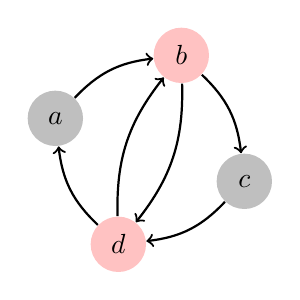
\begin{tikzpicture}[scale=0.8, auto,swap]
			% Draw a 7,11 network
			% First we draw the vertices
			\node[vertex] (a) at (-1,2) {$a$};
			\node[vertex-red] (d) at (1,3) {$b$};
			\node[vertex] (b) at (2,1) {$c$};
			\node[vertex-red] (c) at (0,0) {$d$};
			% Connect vertices with edges and draw weights
			\foreach \source/ \dest in {a/d,d/c,c/d,d/b,b/c,c/a}
				\path[edge] (\source) edge [bend left=20] (\dest);
		\end{tikzpicture}
		\caption{Beispielgraph $g_1$}
	\end{figure}
	\end{minipage}
	\begin{minipage}{0.45\textwidth}
	Eigenschaften von $g_1$:
	\begin{gather*}
		black(g_1, a). \hspace{10pt} arc(g_1, a, b).\\
		red(g_1, b).   \hspace{10pt} arc(g_1, b, c). \\
		black(g_1, c). \hspace{10pt} arc(g_1, c, d). \\
		red(g_1, d).   \hspace{10pt} arc(g_1, d, a). \\
		arc(g_1, d, b).\hspace{10pt} arc(g_1, b, d).
	\end{gather*}
	\end{minipage}
\end{frame}

\begin{frame}
	\frametitle{Appendix - Saturierung (Saturation)}
	Saturierung von $g_1$ mit Hintergrundwissen, dass nur teilweise
	aus \textit{ground literals} besteht:
	\begin{align*}
		\begin{split}
		cyclic(g_1) \leftarrow &\;
		black(g_1, a) , arc(g_1, a, b), red(g_1, b)   , arc(g_1, b, c),\\
		&\;black(g_1, c) , arc(g_1, c, d), red(g_1, d) , arc(g_1, d, a),\\
		&\;arc(g_1, d, b), arc(g_1, b, d), path(g_1, a, c) ,path(g_1, a, c),\\
		&\;path(g_1, a, d) ,path(g_1, b, d) ,path(g_1, b, a) ,path(g_1, c, b),\\
		&\;path(g_1, c, a) ,path(g_1, d, c).
		\end{split}
	\end{align*}
\end{frame}
